\documentclass[aspectratio=169, table]{beamer}

\usepackage{listings}
\usepackage{tikz}
\usetikzlibrary{positioning, arrows.meta, fit}

\usetheme{Pradita}

\title{\Huge Architecture for\\
	\vspace{10pt}
	Big Data Infrastructure}
\subtitle{IT140704 - Big Data for Business}
%\date[Serial]{Penggunaan Large Language Model untuk Pengajaran}
\author{\textbf{Alfa Yohannis}}
\begin{document}
	
	\frame{\titlepage}
	
	
	\begin{frame}[fragile]
		\frametitle{Contents}
		\vspace{20pt}
		\begin{columns}[t]
			\column{0.5\textwidth}
			\tableofcontents[sections={1-6}]
			
			\column{0.5\textwidth}
			\tableofcontents[sections={7-12}]
		\end{columns}
	\end{frame}


\begin{frame}{\hfill}
	\centering
	\Huge{\textbf{What do you think it takes to turn raw data from devices and apps into smart decisions or automation?}}
\end{frame}

	

\section{Introduction}
\begin{frame}[fragile]{Introduction}
	\vspace{20pt}
	\begin{columns}[T]
		% -------- LEFT COLUMN --------
		\column{0.45\textwidth}
		\textbf{Explosion of Digital Data}
		\begin{itemize}
			\item Diverse sources:
			\begin{itemize}
				\item IoT sensors \& smart devices
				\item Social media interactions
				\item E-commerce transactions
				\item IT system logs
			\end{itemize}
			\item Key challenges — the \textbf{3Vs}:
			\begin{itemize}
				\item \textit{Volume}: massive data size
				\item \textit{Velocity}: extremely fast flow
				\item \textit{Variety}: heterogeneous formats
			\end{itemize}
			\item Requires a \textbf{scalable} and \textbf{integrated} architecture.
		\end{itemize}
		
		% -------- RIGHT COLUMN --------
		\column{0.6\textwidth}
		\textbf{Why Big Data Architecture?}
		\begin{itemize}
			\item Connects \emph{acquisition} $\rightarrow$ \emph{storage} $\rightarrow$ \emph{processing} $\rightarrow$ \emph{analytics} $\rightarrow$ \emph{action}.
			\item Enables \textbf{data-driven decision making} while maintaining privacy \& compliance.
			\item \textbf{Layered framework} to be covered:
			\begin{enumerate}
				\item Ingestion \& Raw Data Lake
				\item Processing Layer
				\item Lakehouse / Data Warehouse
				\item BI, ML, \& Operational Systems
				\item Governance \& Orchestration (cross-layer)
			\end{enumerate}
			\item This chapter offers a conceptual overview before diving into each technical layer.
		\end{itemize}
	\end{columns}
\end{frame}

		
	
\section{Architecture}
\begin{frame}[fragile]{Big Data Architecture}
	\vspace{6pt}
	\footnotesize
	\begin{columns}[T,onlytextwidth]
		% --- LEFT COLUMN ---
		\column{0.5\textwidth}
		\textbf{Data Pipeline Layers}
		\begin{itemize}
			\item \textbf{Data Sources:} IoT devices, system logs, APIs, social media
			\item \textbf{Ingestion Layer:} Kafka, Pub/Sub, NiFi — real-time or batch collection
			\item \textbf{Raw Data Lake:} S3, GCS, ADLS, HDFS — stores unstructured, semi-structured data
			\item \textbf{Processing:} Spark, Flink, Dataflow — cleansing, transformation, aggregation
			\item \textbf{Lakehouse / DW:} BigQuery, Snowflake, Delta Lake — structured, queryable storage
		\end{itemize}
		
		% --- RIGHT COLUMN ---
		\column{0.5\textwidth}
		\textbf{Consumption \& Governance}
		\begin{itemize}
			\item \textbf{BI \& Analytics:} Tableau, Power BI, Looker — dashboards, KPIs, reports
			\item \textbf{Machine Learning:} SageMaker, TensorFlow, Feature Store — model training, inference
			\item \textbf{Operational Systems:} Recommenders, alerts, automation
			\item \textbf{Governance \& Orchestration:} Atlas, Airflow, IAM, Data Catalog — quality, security, lineage
		\end{itemize}
	\end{columns}
\end{frame}


	
	
	\begin{frame}[fragile]{Big Data Architecture Diagram}
		\vspace{20pt}
		\begin{center}
		\scalebox{0.7}{
			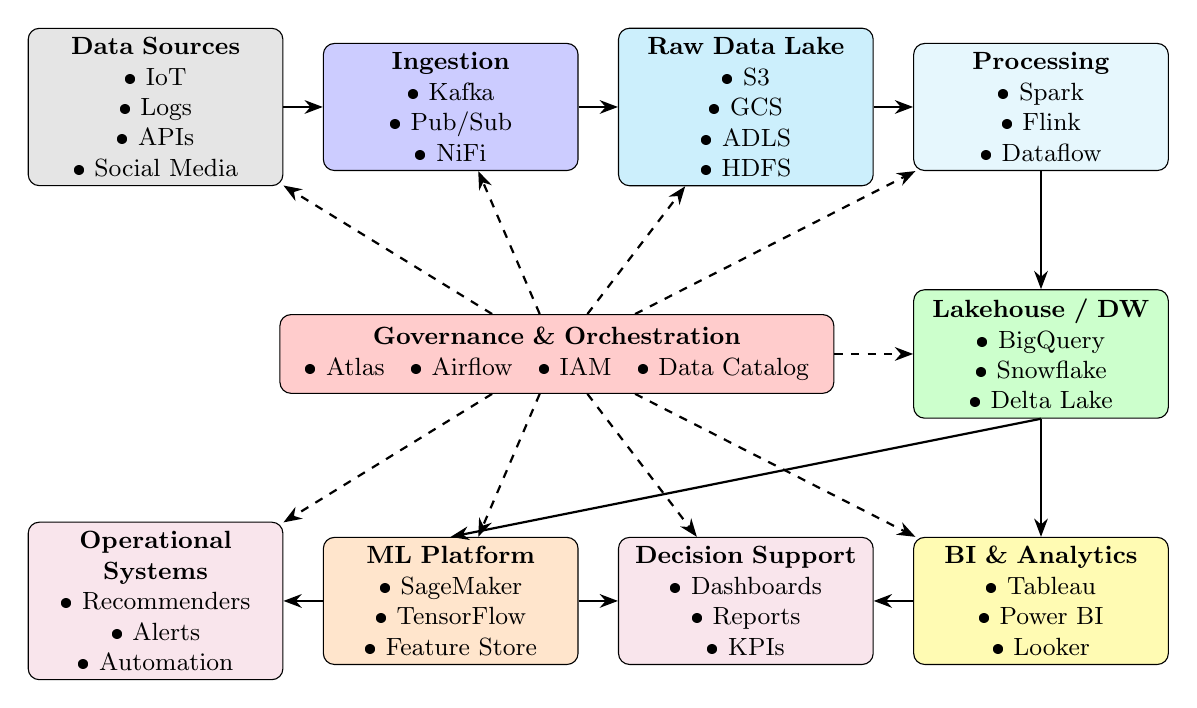
\begin{tikzpicture}[node distance=1cm and 0.5cm]
				% ----- Styles -----
				\tikzset{
					box/.style={
						rectangle, draw, rounded corners,
						minimum width=2.2cm, minimum height=1cm,
						text width=3cm, align=center, font=\small
					},
					widebox/.style={
						rectangle, draw, rounded corners,
						minimum width=6.5cm, minimum height=1cm,
						text width=6.8cm, align=center, font=\small
					},
					source/.style={box, fill=gray!20},
					ingestion/.style={box, fill=blue!20},
					storage/.style={box, fill=cyan!20},
					processing/.style={box, fill=cyan!10},
					lakehouse/.style={box, fill=green!20},
					serving/.style={box, fill=yellow!30},
					ml/.style={box, fill=orange!20},
					governance/.style={widebox, fill=red!20},
					output/.style={box, fill=purple!10},
					arrow/.style={thick, ->, >=Stealth},
					dashedarrow/.style={thick, dashed, ->, >=Stealth}
				}
				% ----- Nodes -----
				\node (source)    [source]        {\textbf{Data Sources}\\• IoT\\• Logs\\• APIs\\• Social Media};
				\node (ingest)    [ingestion, right=of source] {\textbf{Ingestion}\\• Kafka\\• Pub/Sub\\• NiFi};
				\node (lake)      [storage, right=of ingest]   {\textbf{Raw Data Lake}\\• S3\\• GCS\\• ADLS\\• HDFS};
				\node (process)   [processing, right=of lake]  {\textbf{Processing}\\• Spark\\• Flink\\• Dataflow};
				
				\node (warehouse) [lakehouse, below=1.5cm of process] {\textbf{Lakehouse / DW}\\• BigQuery\\• Snowflake\\• Delta Lake};
				
				\node (gov) [governance, left=1cm of warehouse] {\textbf{Governance \& Orchestration}\\• Atlas\quad• Airflow\quad• IAM\quad• Data Catalog};
				
				\node (bi)       [serving, below=1.5cm of warehouse] {\textbf{BI \& Analytics}\\• Tableau\\• Power BI\\• Looker};
				\node (decision) [output, left=.5cm of bi]   {\textbf{Decision Support}\\• Dashboards\\• Reports\\• KPIs};
				
				\node (ml)       [ml, left=of decision]      {\textbf{ML Platform}\\• SageMaker\\• TensorFlow\\• Feature Store};
				\node (opsys)    [output, left=.5cm of ml]   {\textbf{Operational Systems}\\• Recommenders\\• Alerts\\• Automation};
				
				% ----- Arrows -----
				\draw[arrow] (source) -- (ingest);
				\draw[arrow] (ingest) -- (lake);
				\draw[arrow] (lake)   -- (process);
				\draw[arrow] (process) -- (warehouse);
				
				\draw[arrow] (warehouse.south) -- (bi.north);
				\draw[arrow] (warehouse.south) -- (ml.north);
				\draw[arrow] (bi) -- (decision);
				\draw[arrow] (ml) -- (opsys);
				\draw[arrow] (ml) -- (decision);
				
				% Governance dashed arrows
				\foreach \t in {source, ingest, lake, process, warehouse, bi, ml, decision, opsys}{
					\draw[dashedarrow] (gov) -- (\t);
				}
			\end{tikzpicture}
		}
	\end{center}
	\end{frame}
	
	\section{Data Sources}
	\begin{frame}[fragile]{Data Sources in Big Data}
		\vspace{20pt}
		\textit{Data sources} are the origins from which raw information enters a big data system. These vary in structure, speed, and value, forming the foundation of data-driven insights.
		
		\vspace{6pt}
		\begin{columns}[T,onlytextwidth]
			\column{0.55\textwidth}
			\textbf{Types of Data Sources}
			\begin{itemize}
				\item \textbf{IoT Devices:} sensors, health monitors, CCTV, factory machines.
				\item \textbf{System Logs:} records of logins, activity, and system responses.
				\item \textbf{APIs:} bridges to external apps—stock data, weather, maps.
				\item \textbf{Social Media:} text, images, videos from platforms like Twitter.
			\end{itemize}
			
			\column{0.45\textwidth}
			\textbf{Key Characteristics}
			\begin{itemize}
				\item Real-time, batch, or event-driven.
				\item Structured to unstructured formats.
				\item High volume, varying frequency, diverse formats.
				\item Need scalable and reliable ingestion systems.
			\end{itemize}
		\end{columns}
	\end{frame}
	
	
	\begin{frame}[fragile]{Ingestion Layer}
		\vspace{20pt}
		The \textbf{ingestion layer} is the entry point of big data architecture, capturing and transferring data from sources like IoT devices, system logs, APIs, and social media into central storage (e.g., a data lake). Due to the continuous and fast nature of incoming data, this layer needs reliable and efficient tools. \textit{\textbf{Analogy:}} Like the main gate of a data warehouse—directing all incoming data without delay or loss.
		
		\vspace{6pt}
		\textbf{Common Ingestion Technologies:}
		\begin{itemize}
			\item \textbf{Apache Kafka}: Real-time, scalable message queue using a publish-subscribe model.
			\item \textbf{Google Cloud Pub/Sub}: Cloud-based service for asynchronous, distributed messaging.
			\item \textbf{Apache NiFi}: Visual tool for building secure, monitored data pipelines without coding.
		\end{itemize}
	\end{frame}
	
	

	\section{Raw Data Lake}
	
	\begin{frame}[fragile]{Raw Data Lake}
		\vspace{20pt}
		A \textbf{raw data lake} is a central repository for storing all incoming data—structured or unstructured—in its original form. Like water into a lake, data flows in without filtering. These systems support real-time/batch access, security, versioning, and governance. \textbf{Key benefits:} Flexibility and scalability, allowing data to be stored now and analyzed later.
		
		\vspace{6pt}
		\textbf{Technologies:}
		\begin{itemize}
			\item \textbf{Amazon S3}: Scalable storage with fast access and ML support.
			\item \textbf{Google Cloud Storage (GCS)}: Petabyte-scale storage for analytics.
			\item \textbf{Azure ADLS}: Big data storage with broad format support.
			\item \textbf{Hadoop HDFS}: Distributed system for large-scale parallel storage.
		\end{itemize}
	\end{frame}
	
	
	\section{Processing Layer}
	
	\begin{frame}[fragile]{Processing Layer}
		\vspace{20pt}
		The \textbf{processing layer} transforms raw data from the data lake into clean, structured, and usable information. It handles tasks like cleansing, transformation, aggregation, and labeling for analytics or ML. \textit{Analogy:} Like a kitchen preparing raw ingredients into ready-to-serve meals.
		
		\vspace{6pt}
		\textbf{Processing Modes:}
		\begin{itemize}
			\item \textbf{Batch:} Periodic large-scale processing (e.g., hourly/daily reports).
			\item \textbf{Streaming:} Real-time processing for immediate use (e.g., fraud detection).
		\end{itemize}
		
		\vspace{4pt}
		\textbf{Technologies:}
		\begin{itemize}
			\item \textbf{Apache Spark:} Unified engine for batch and stream processing with ML libraries.
			\item \textbf{Apache Flink:} Low-latency engine specialised in real-time stream processing.
			\item \textbf{Google Cloud Dataflow:} Cloud-native engine supporting Apache Beam pipelines.
		\end{itemize}
	\end{frame}
	
	\section{Lakehouse and Data Warehouse}
	
	\begin{frame}[fragile]{Lakehouse and Data Warehouse}
		\vspace{20pt}
		\begin{columns}[T,onlytextwidth]
			\column{0.5\textwidth}
			\textbf{Concepts and Benefits}
			\begin{itemize}
				\item \textbf{Data Warehouse:} Structured archive for reporting. Requires clean, curated data.
				\item \textbf{Lakehouse:} Hybrid approach—raw and structured data in one layer.
				\item Reduces duplication, accelerates analytics, supports ML workflows.
				\item Ensures trusted, analysis-ready data for BI and AI use.
			\end{itemize}
			
			\column{0.5\textwidth}
			\textbf{Popular Platforms}
			\begin{itemize}
				\item \textbf{BigQuery:} Scalable cloud SQL engine for large-scale analysis.
				\item \textbf{Snowflake:} Multi-format warehouse with elastic compute and secure data sharing.
				\item \textbf{Delta Lake:} ACID-compliant lakehouse for batch and streaming on Spark.
			\end{itemize}
		\end{columns}
	\end{frame}
	
	
	\section{BI and Analytics}
	
	\begin{frame}[fragile]{BI \& Analytics Layer}
		\vspace{20pt}
		\begin{columns}[T,onlytextwidth]
			% ---------- LEFT 50% ----------
			\column{0.5\textwidth}
			\textbf{Purpose and Benefits}
			\begin{itemize}
				\item Turns processed data into dashboards, reports, and interactive visuals.
				\item Enables quick, data-driven decisions for managers and analysts.
				\item Reveals hidden patterns and business trends.
			\end{itemize}
			
			% ---------- RIGHT 50% ----------
			\column{0.5\textwidth}
			\textbf{Popular BI Tools}
			\begin{itemize}
				\item \textbf{Tableau:} Drag-and-drop dashboards, connects to many data sources.
				\item \textbf{Power BI:} Microsoft ecosystem, strong Excel and Azure integration.
				\item \textbf{Looker:} Model-driven web BI on Google Cloud, centralised business logic.
			\end{itemize}
		\end{columns}
	\vspace{10pt}
	\textbf{Analogy:} Like a car’s dashboard—showing key metrics (speed, fuel, warnings) at a glance.\textbf{Accurate data} and the right BI tool turns raw information into real business value—boosting efficiency, customer insights, and strategic planning.
	
	\end{frame}
	
	\section{Machine Learning Platform}
	
	\begin{frame}[fragile]{Machine Learning (ML) Layer}
		\vspace{20pt}
		\begin{columns}[T,onlytextwidth]
			% ---------- LEFT 50% ----------
			\column{0.5\textwidth}
			\textbf{Purpose and Role}
			\begin{itemize}
				\item Builds predictive/classification models from processed historical data.
				\item Enables automated decisions—e.g., fraud detection, demand forecasting.
				\item \textit{Analogy:} Like an R\&D division—studies past data to plan smarter strategies.
			\end{itemize}
			ML platforms support the full model lifecycle: training, validation, deployment, and prediction delivery.
			
			% ---------- RIGHT 50% ----------
			\column{0.5\textwidth}
			\textbf{Key Technologies}
			\begin{itemize}
				\item \textbf{Amazon SageMaker:} Full-stack ML service for fast model development and deployment.
				\item \textbf{TensorFlow:} Widely used open-source framework for scalable ML and deep learning.
				\item \textbf{Feature Store:} Central repository to store and manage features for consistent model training and serving.
			\end{itemize}
			Successful ML implementation requires infrastructure, collaboration, and alignment with business goals.
		\end{columns}
	\end{frame}
	
	
	\section{Decision Support}
	
	\begin{frame}[fragile]{Decision Support Layer}
		\vspace{20pt}
		\begin{columns}[T,onlytextwidth]
			% ---------- LEFT 50% ----------
			\column{0.5\textwidth}
			\textbf{Purpose and Role}
			\begin{itemize}
				\item Transforms analysed data into actionable insights.
				\item Supports strategic, tactical, and operational decisions.
				\item \textit{Analogy:} Like a dashboard in a car—simplifies internal operations into key signals for decision-makers.
			\end{itemize}
			Integration with analytics, processing, and governance layers ensures relevant and timely insights.
			
			% ---------- RIGHT 50% ----------
			\column{0.5\textwidth}
			\textbf{Typical Outputs}
			\begin{itemize}
				\item \textbf{Dashboards:} Real-time visuals showing KPIs, trends, and alerts.
				\item \textbf{Reports:} Structured periodic summaries for different management levels.
				\item \textbf{KPIs:} Metrics to measure business goal achievement (sales, satisfaction, conversion rate).
			\end{itemize}
			Reliable decision support bridges technical data work with impactful business decisions.
		\end{columns}
	\end{frame}
	
	\section{Operational Systems}
	
	\begin{frame}[fragile]{Operational Systems Layer}
		\vspace{20pt}
		\begin{columns}[T,onlytextwidth]
			% ---------- LEFT 50% ----------
			\column{0.5\textwidth}
			\textbf{Role and Analogy}
			\begin{itemize}
				\item Supports real-time, automated operational responses.
				\item Focuses on day-to-day execution, not high-level decisions.
				\item \textit{Analogy:} Like an autopilot system—responds instantly to sensor data without human input.
			\end{itemize}
			Enables data-driven operations that are fast, scalable, and adaptive.
			
			% ---------- RIGHT 50% ----------
			\column{0.5\textwidth}
			\textbf{Common Implementations}
			\begin{itemize}
				\item \textbf{Recommender Systems:} Suggest products or content based on user behaviour.
				\item \textbf{Alerts \& Notifications:} Auto-detect anomalies like fraud or system failure.
				\item \textbf{Process Automation:} Auto-schedule, auto-reply, or auto-adjust based on real-time data.
			\end{itemize}
			Strong integration of real-time data, analytics, and business logic is essential for reliability.
		\end{columns}
	\end{frame}
	
	\section{Governance and Orchestration}
	
	\begin{frame}[fragile]{Governance and Orchestration Layer}
		\vspace{20pt}
		\begin{columns}[T,onlytextwidth]
			% ---------- LEFT COLUMN ----------
			\column{0.5\textwidth}
			\textbf{Purpose and Role}
			\begin{itemize}
				\item Ensures data quality, security, and compliance.
				\item Manages workflow execution across the data pipeline.
				\item \textit{Analogy:} Like traffic control—enforcing rules, timing, and order in data movement.
			\end{itemize}
			Promotes trust, accountability, and auditability across the data lifecycle.
			
			% ---------- RIGHT COLUMN ----------
			\column{0.5\textwidth}
			\textbf{Key Tools}
			\begin{itemize}
				\item \textbf{Apache Atlas:} Metadata manager for lineage, classification, and policy.
				\item \textbf{Apache Airflow:} Workflow scheduler for managing complex data pipelines.
				\item \textbf{IAM (Identity \& Access Management):} Controls data access rights per user.
				\item \textbf{Data Catalog:} Searchable index of all data assets across the organisation.
			\end{itemize}
			Enables efficient, secure, and compliant data operations.
		\end{columns}
	\end{frame}
	
	\section{End-to-End Data Flow}
	
	%------------------------------------------------
	% Frame — End-to-End Data Flow (no columns)
	%------------------------------------------------
	\begin{frame}[fragile]{End-to-End Data Flow}
		\vspace{20pt}
		\textbf{Main Steps}
		\begin{enumerate}
			\item \textbf{Ingestion} — Collect data via Kafka, NiFi, APIs.
			\item \textbf{Raw Data Lake} — Store unfiltered data in S3, GCS.
			\item \textbf{Processing} — Clean\slash transform with Spark or Flink (batch \& streaming).
			\item \textbf{Lakehouse / DW} — Load curated data into Delta Lake, BigQuery.
			\item \textbf{Consumption} — BI dashboards or ML platforms generate insights.
			\item \textbf{Action} — Dashboards for managers or real-time triggers for ops systems.
			\item \textbf{Governance \& Orchestration} — Atlas, Airflow, IAM secure and automate flow.
		\end{enumerate}
		
		\vspace{10pt}
		\textbf{Analogy:} Like a supply chain—raw materials (data) enter, get processed, and are delivered as finished products (insights or automation). Each step depends on the one before it, ensuring smooth flow, traceability, and value delivery from source to impact.
	\end{frame}
	
	
%------------------------------------------------
% Frame 1 — Use Case: Fraud Detection
%------------------------------------------------
\begin{frame}[fragile]{Fraud Detection in Financial Transactions}
	\vspace{10pt}
	A financial institution collects customer transaction data in real-time via APIs and system logs. The raw data is stored in \textbf{Google Cloud Storage}. Data processing is performed using \textbf{Apache Flink} to detect suspicious transaction patterns on the fly.
	
	\vspace{10pt}
	Once processed, the results are stored in \textbf{Snowflake} and consumed by a \textbf{machine learning model} to classify potential fraud cases. If a transaction receives a high-risk score, the system automatically triggers a \textbf{notification} to the security team and temporarily halts the transaction for manual verification.
	
	\vspace{10pt}
	All steps are coordinated and logged using \textbf{Airflow}, while \textbf{Data Catalog} and \textbf{IAM} ensure access control is maintained only for authorised personnel.
\end{frame}

%------------------------------------------------
% Frame 2 — Use Case: Sentiment Analysis for Marketing
%------------------------------------------------
\begin{frame}[fragile]{Sentiment Analysis for Marketing Strategy}
	\vspace{10pt}
	An e-commerce company monitors reviews and comments from social media platforms (e.g., Twitter and Instagram) through API connections. The data is collected using \textbf{Apache NiFi} and stored in a data lake based on \textbf{Amazon S3}.
	
	\vspace{10pt}
	\textbf{Natural Language Processing (NLP)} is performed using \textbf{Apache Spark} to extract sentiment and key themes. This information is loaded into \textbf{Delta Lake} and visualised through a dashboard built with \textbf{Power BI}.
	
	\vspace{10pt}
	The marketing team leverages these insights to adjust promotional strategies in real-time. The entire pipeline is orchestrated using \textbf{Airflow} and monitored by \textbf{Apache Atlas} for metadata tracking and auditability.
\end{frame}

	
\begin{frame}[fragile]{Conclusion}
	\vspace{20pt}
	\begin{itemize}
		\item Big data architecture integrates components from ingestion, storage, processing, and consumption.
		\item Raw data is collected and stored in scalable data lakes before being processed into structured formats.
		\item Processed data is consumed through BI dashboards, machine learning models, and operational systems.
		\item Governance and orchestration layers ensure the entire flow is secure, scheduled, and compliant.
		\item This end-to-end system allows organisations to transform large volumes of data into actionable insights.
	\end{itemize}
\end{frame}

	
	
	%\section{Bab 1: Pengenalan ChatGPT}
	%\begin{frame}{\hfill}
	%	\centering
	%	\Huge{\textbf{Bab 1: Pengenalan ChatGPT}}
	%\end{frame}	
\end{document}
